\subsection{Βήμα 1ο - Δεδομένα από IMDb}
Με τις ρυθμίσεις που του
%ποιανού
δόθηκαν για αυτήν την πτυχιακή αρχικά παίρνει
%ποιός
ένα συμπιεσμένο αρχείο με δεδομένα βαθμολογιών ταινιών από το IMDb το αποσυμπιέζει και αποθηκεύει τα δεδομένα στην μνήμη. Η Μορφή
%Το περιεχόμενο?
δεδομένων του αρχείου είναι: το αναγνωριστικό μιας ταινίας η μιας σειράς (imdbId), η βαθμολογία της ταινίας/σειράς (rating) καθώς και το νούμερο των ψήφων με το οποίο βγήκε αυτή η βαθμολογία (voteCount). Έπειτα παίρνει ένα ακόμα συμπιεσμένο αρχείο από το IMDb του οποίου η μορφή
%..το οποίο περιέχει..
είναι το αναγνωριστικό μιας ταινίας η μιας σειράς (imdbId) και ο τύπος (titleType). Δηλαδή
%Ο τύπος διευκρινίζει εάν
αν είναι ταινία, σειρά ή κάτι άλλο. 

Αφού φορτώσει και τα 2 αρχεία στη μνήμη ξεχωρίζει τις εγγραφές που αναφέρουν μόνο ταινίες και μετά ξεχωρίζει τις εγγραφές οι οποίες έχουν αριθμό ψήφων μεγαλύτερο ή ίσο με μια σταθερά MINIMUM\_VOTES\_THRESHOLD και κρατάει τα 3 αρχικά πεδία του πρώτου αρχείου. Η Σταθερά αυτή για αυτό το σενάριο είναι 1000.
%σενάριο
%Η σταθερά αυτή έχει καθοριστεί ως 1000 ψήφοι.
%discard entry process
%σύνδεση με 2ο βήμα

\begin{figure}[h]
  \centering
  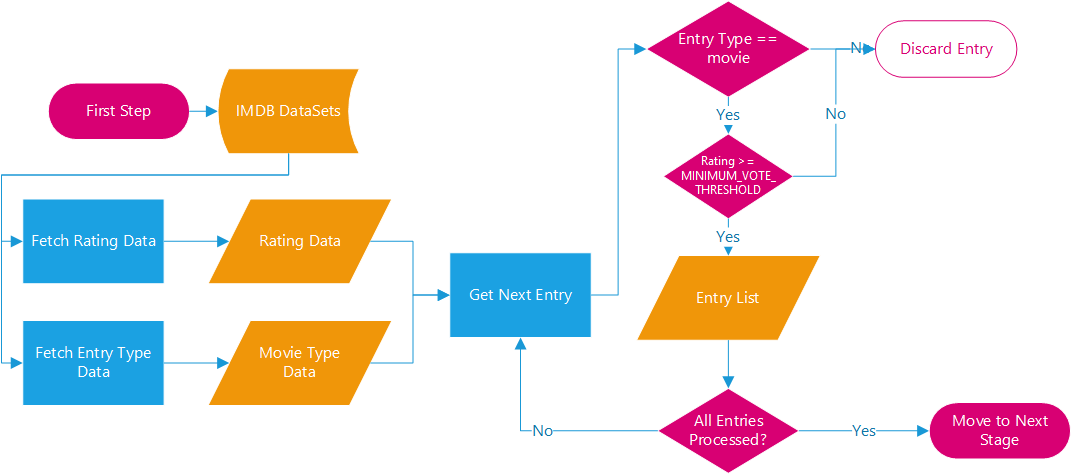
\includegraphics[width=150mm]{Chapters/5 - Architecture/Import/Images/imdb_flowchart.png}
  \caption{Διάγραμμα ροής δεδομένων από IMDB}
  \label{flowchart:imdbImport}
\end{figure}